\chapter{Results}
\label{chp:results} 

\section{Introduction}

This chapter presents how the robot and the supporting implementations were tested and the results that where obtained. The same software system was used for both the simulated and live robot. It was still necessary to have some separate launch and configuration files for the simulated and hardware version (section \ref{sec:integration}). Section \ref{sec:testplan} provides an overview of the various features and components which were tested, and how these items are assessed. Next, in section \ref{sec:results_summary}, a brief overview of the results are presented. The two last sections will go through the more nuanced results and events from the simulations and live trials respectively. It was difficult to come up with a rigorous test plan because of time constraints. Much of the testing was done together with parameter tuning. 


\section{Testplan}
\label{sec:testplan}
The tests listed in tables \ref{tab:support_func} and \ref{tab:main_func} will be carried out in the simulator, as well as in the real world. They will mainly focus on the navigation stack and \ac{RTAB-Map}. 

\begin{table}
	\centering
	\begin{tabular}{ p{3.5cm} | p{7cm} }
		\multicolumn{2}{c}{Supporting Functionality}\\
		\hline
		\textbf{Evaluate} & Description\\
		\hline
		\textbf{Mobile application, ''Robot Leash''} & Use the mobile application to manually steer the robot.\\
		\hline
		\textbf{Operator Control Station} & Steer the robot from the \ac{OCS} while monitoring the robot through the live video stream. \\
		\hline
		\textbf{Motor controller on XMEGA A3BU} & Verify ability to command the wheels. Confirm that the vehicle stops when velocity commands from \ac{ROS} are absent.\\
		\hline
	\end{tabular}
	\caption{Supporting Functionality}\label{tab:support_func}
\end{table}

\begin{table}
	\centering
	\begin{tabular}{ p{2.5cm} | p{7cm} }
	\multicolumn{2}{c}{Core Functionality}\\
\hline
	\textbf{Evaluate} & Description\\
	\hline
	\textbf{Multi Session Mapping} & Verify that the robot can rediscover areas which have been mapped in a previous mapping session.\\
	\hline
	\textbf{Loop Closure Detection} & As a core functionality in \ac{RTAB-Map}, it is critical to evaluate the loop closure mechanism.\\
	\hline
	\textbf{Autonomous Navigation} & Perform a set of tests on the navigation stack. The tests should evaluate path planning with moving obstacles. Different parameters should be tested and evaluated. Observe how the robot handles narrow passages. Evaluate robustness of the navigation stack for this robot.\\
	\hline
	%\caption{}
	\end{tabular}
	\caption{Core Functionality}\label{tab:main_func}
\end{table}

\section{Brief Summary of All Results}
\label{sec:results_summary}
%\begin{table}
%	\centering
%	\begin{tabular}{ p{3.5cm} | p{7cm} }
%		\multicolumn{2}{c}{Result Summary}\\
%		\hline
%		\textbf{Test Item} & Evaluation\\
%		\hline
%		\textbf{Mobile application, ''Robot Leash''} & The mobile App works as expected. The user can connect to the robot and send velocity commands to the real and simulated mobile base via Bluetooth. This tool proved to be invaluable, and was used during all mapping sessions.\\
%		\hline
%		\textbf{Multi Session Mapping} & An example of multi session mapping was recorded to the video \texttt{live\_multi\_session\_mapping} enclosed in the DVD. The live robot can successfully merge multiple maps. In Gazebo, the method is more vulnerable to similar features in different parts of the world.\\
%		\hline
%		\textbf{Loop Closure Detection} & Successful live loop closure detection is demonstrated in the video \texttt{live\_mapping\_succesful}. The simulated environment was a bit more challenging, as demonstrated in the enclosed video \texttt{sim\_wrong\_loop\_closure}.\\
%		\hline
%		\textbf{Autonomous Navigation} & Autonomous navigation was evaluated based on the ability to reach a feasable goal state, and the ability to avoid static and dynamic obstacles. The global planner works as expected in both the simulator and in the real world. The simulated robot was frequently unable to reach its goal. The real robot successfully navigated a static and dynamic obstacle course (video \texttt{live\_navigation\_1} and \texttt{2}, and ''Obstruction detection and avoidance'').\\
%		\hline
		%\caption{}
%	\end{tabular}
%	\caption{Result Summary}\label{tab:result}
%\end{table}

\subsubsection{Mobile application, ''Robot Leash''}

The mobile App works as expected. The user can establish a Bluetooth connection to the robot and send velocity commands to the real and simulated mobile base. This tool proved to be invaluable, and was used during all mapping sessions, both real and simulated.

\subsubsection{Operator Control Station}

\subsubsection{Motor controller on XMEGA A3BU}

An example of multi session mapping was recorded to the video ''\texttt{live\_multi\_session\_mapping}'' enclosed in the DVD. The live robot can successfully merge multiple maps. In Gazebo, the method is more vulnerable to similar features in different parts of the world.

\subsubsection{Loop Closure Detection}

Successful live loop closure detection is demonstrated in the video ''\texttt{live\_mapping\_succesful}''. The simulated environment was a bit more challenging, as demonstrated in the enclosed video ''\texttt{sim\_wrong\_loop\_closure}''.

\subsubsection{Autonomous Navigation}

Autonomous navigation was evaluated based on the ability to reach a feasable goal state, and the ability to avoid static and dynamic obstacles. The global planner works as expected in both the simulator and in the real world. The simulated robot was frequently unable to reach its goal. The real robot successfully navigated a static and dynamic obstacle course (video ''\texttt{live\_navigation\_1}'' and \texttt{2}, and ''Obstruction detection and avoidance'').



\section{Simulation Results}

The system was tested on a simulated model of the robot in Gazebo. A simulated environment, \texttt{Asphalt.world} shown in figure \ref{fig:gazebo2_cropped}, was populated with objects and clutter in order to provide a test environment with distinctive visual features for the visual mapping approach, and obstacles for the navigation stack. 
%An included simulator world of the Willow Garage office building was considered as a testing area. Unfortunately, the gray hallways and offices did not provide enough good visual features for \ac{RTAB-Map}.

\begin{figure}[h]
	\centering
	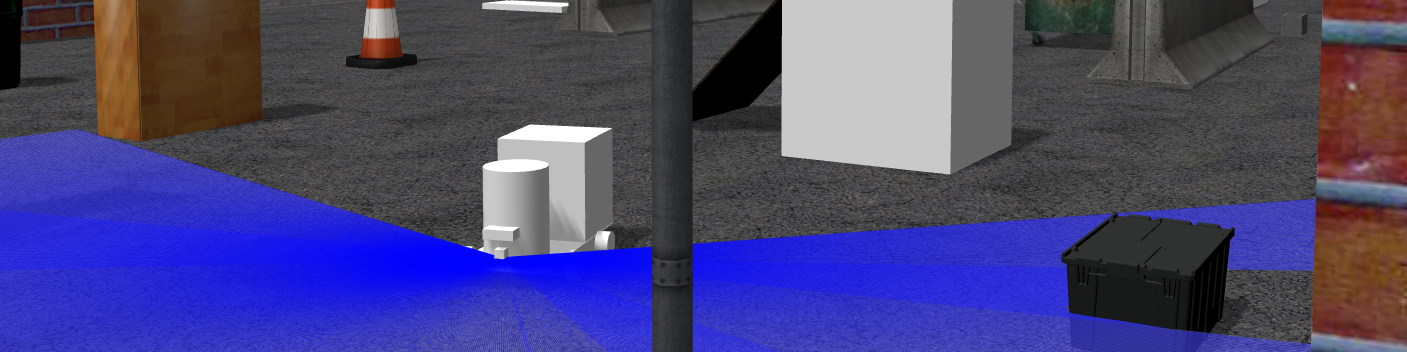
\includegraphics[width=1\textwidth]{gazebo2_cropped}
	\caption{The ''Asphalt'' world in Gazebo. }
	\label{fig:gazebo2_cropped}
\end{figure}

\subsection{Mapping}

\ac{RTAB-Map} on the robot in Gazebo allowed controlled testing of edge cases in a controlled environment. The ''Asphalt'' world proved to be a challenge for \ac{RTAB-Map} - at least with the parameters that were used during testing. Figure \ref{fig:rviz_mapping_trial} shows an example of a resulting 3D map. 

\begin{figure}[h]
	\centering
	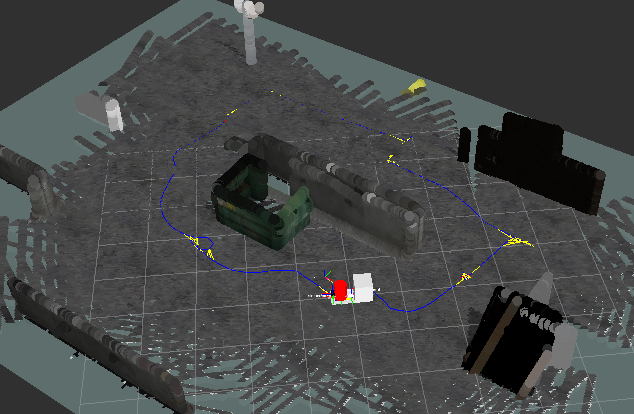
\includegraphics[width=0.7\textwidth]{rviz_mapping_trial_cropped}
	\caption{An example of a resulting point cloud map after running \ac{RTAB-Map} in Gazebo. }
	\label{fig:rviz_mapping_trial}
\end{figure}

The map quality varied greatly between the mapping trials. The path of the robot was found to have a significant impact on the recorded path between the stored locations in the \ac{RTAB-Map} system. An example of a problematic path is to drive the robot in parallel to a wall. Such a path creates few or none distinctive features as long as the robot follows this path. Figure \ref{fig:gazebo_lc_features} shows two problematic events. First, a loop closure is detected based on similarities detected on the asphalt plane. Because the loop closure is wrong, a wrong pose transform correction will be propagated backwards along the path of the robot, ultimately resulting in a displaced map.

\begin{figure}[h]
	\centering
	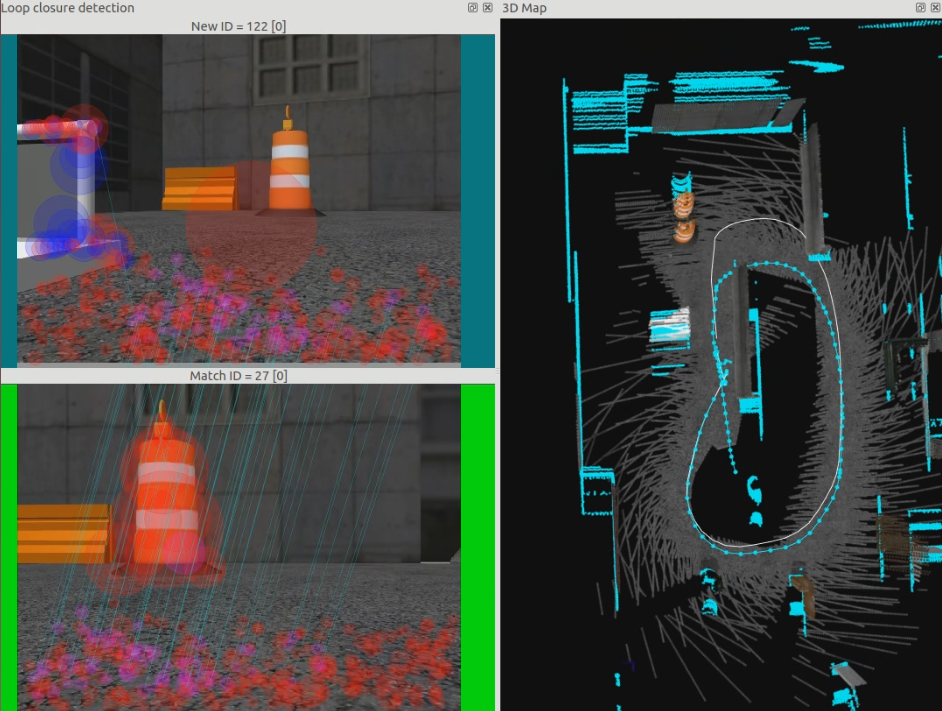
\includegraphics[width=0.9\textwidth]{gazebo_lc_features}
	\caption{Example of an incorrect loop closure detection. The pink circles indicate matching features. The right part shows an incorrect map adjustment. Observe how the matching features are located on the asphalt plane.}
	\label{fig:gazebo_lc_features}
\end{figure}

\begin{figure}[h]
	\centering
	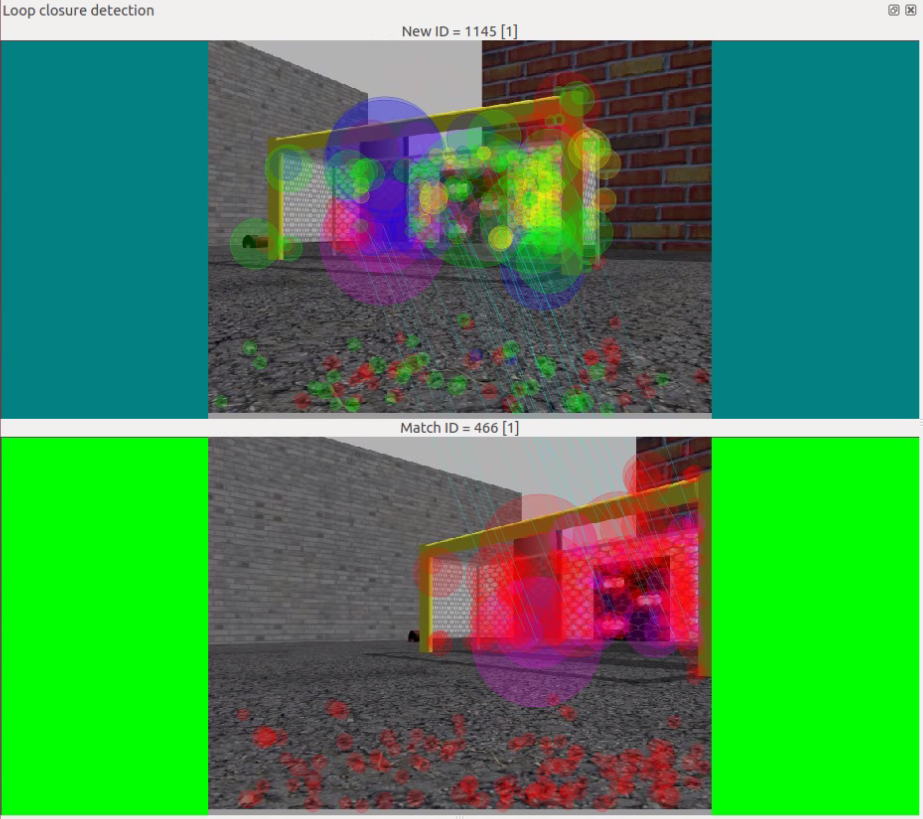
\includegraphics[width=0.9\textwidth]{loop_closure_detection}
	\caption{An example of an accepted and correct loop closure hypothesis. This example is from the ''Asphalt'' world simulated in Gazebo.}
	\label{fig:loop_closure_detection}
\end{figure}

Another error occurred during a multi session mapping trial. The robot detected a wrong loop closure at a location with similar features to a previously mapped location. This resulted in the map seen in figure \ref{fig:Incorrect_lc_detection}. Other localization problems were apparent when driving in open areas. The estimated location of the robot would fluctuate when turning the robot as features passed in or out of view.

Sensor settings is another factor that had a high impact on the \ac{SLAM} quality. When sensor ranges of the Gazebo sensor plugins are set according to the sensors technical specifications, both localization and mapping will struggle. An increased sensor range in for the simulated sensors would increase the \ac{SLAM} robustness.

\begin{figure}[h]
	\centering
	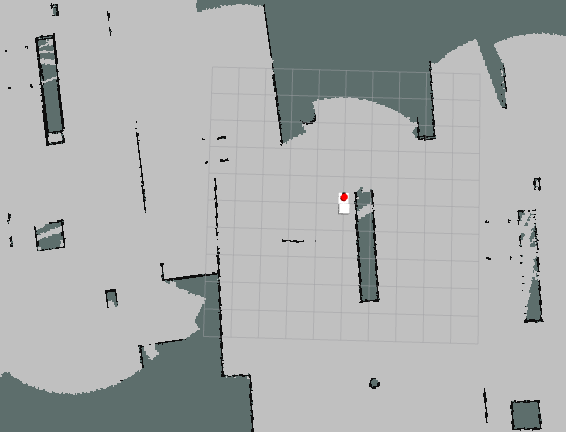
\includegraphics[width=0.75\textwidth]{Incorrect_lc_detection_cropped}
	\caption{An example of incorrect map merging. This case occurred in the ''Asphalt'' world simulated in Gazebo.}
	\label{fig:Incorrect_lc_detection}
\end{figure}


\subsection{Autonomous Navigation}

Testing the navigation stack in Gazebo fulfilled two goals. The first goal was to learn how the system behaved with different parameters and to uncover potential problems with the system before attempting to test the live robot. The second goal was to evaluate the ability to relocate the robot and avoid obstacles. 

The for the first trial, the robot footprint was extended well beyond the physical mobile base. The purpose of this was to prevent obstacles from getting too close to the Kinect and \ac{LIDAR}. As the minimum detectable range for the Kinect is $0.5 m$ (measured minimum depth), the footprint was extended $0.5 m$ beyond the front of the mobile base. A second parameter to be tuned is the obstacle inflation radius, i.e. the radius beyond each obstacle that is expensive or impossible to traverse. Figure \ref{fig:big_footprint} illustrates both the big footprint and the obstacle inflation radius.

During trials with the big footprint, the robot showed good collision avoidance capabilities but an aversion to narrow passages. Setting the obstacle inflation radius is also a dilemma in choosing between large margins for the global path or the ability to navigate through narrow passages. 

\begin{figure}[h]
	\centering
	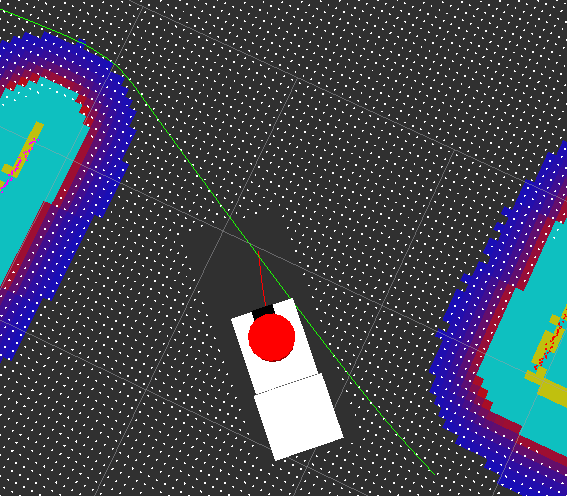
\includegraphics[width=0.7\textwidth]{planning_big_footprint_cropped}
	\caption{The robot footprint is illustrated by the clear rectangle that surrounds the robot model. The coloured areas are map locations with high cost. }
	\label{fig:big_footprint}
\end{figure}

In later navigation sessions, the robot footprint was reduced to a size slightly larger than the physical robot base. During some of the testing sessions, the robot would get stuck near obstacles. 

Sometimes, the robot would never actually reach the goal state, but rather circle around it. This problem was not solved, but more relaxed goal tolerances mitigated the issue a little. 

\section{Live Robot Results}

Due to time constraints, it was no time to tune the parameters of \ac{RTAB-Map}. \ac{RTAB-Map} is therefore used with the default parameters. An important distinction between the real and simulated system is found in the actuator, i.e. the motor controller of the mobile base. In the simulated system, the motor control card is emulated by a skid steering plugin. While the exact functionality of the skid steering plugin is unknown, it does ensure that the wheels follow the linear and angular velocity commands provided by \ac{ROS}. This is not the case for the real motor control card, as it lacks a feedback loop. The real robot velocity was in general slower that its simulated version.

\subsubsection{Safety Features}

The simulator offered the benefit of a risk free environment. This is not the case for the real robot. 

\subsubsection{Loop Closure Detection}

Loop closure detection was carried out on the first floor of Gamle Elektro at Gløshaugen, NTNU (figure \ref{fig:mapping_gamle_elektro}). This environment provides a good mix of featureless and feature rich surroundings. It will also provide an additional challenge because of the many students that use the hallways. Most importantly, there are loops in the environment that allow testing of vision based loop closures and odometry error correction. 

The first test run revealed two problems with the implementation, the first being odometry errors and the second being a failure to visually detect loop closures. Odometry based on laser scans would wrongfully indicate a change in the robot heading in some cases, and in other cases fail to correctly indicate heading changes when rounding corners. 

In later experiments it was found that different mapping techniques and path choices could either prevent or cause odometry errors. It was also found that it is helpful to start a mapping session in an area that is rich in distinctive features. The map and floor plan comparison shown in figure \ref{fig:comparison} shows a map where a loop closure was successfully detected. In the same figure, notice how the upper hallway is misaligned to the rest of the map. The robot failed to detect any good visual features in this area. Figure \ref{fig:lc_match_live} shows the resulting point cloud map of the same area.

\begin{figure}
	\centering
	\begin{subfigure}[b]{1\textwidth}
		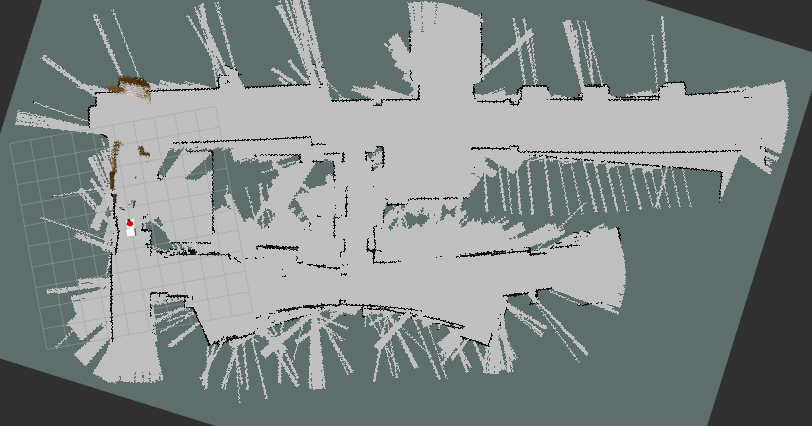
\includegraphics[width=\textwidth]{mapping_gamle_elektro}
		\caption{Resulting occupancy grid after a mapping session. The mapping  method is struggling with the  hallway in the upper part of the image.}
		\label{fig:mapping_gamle_elektro}
	\end{subfigure}
	\begin{subfigure}[b]{1\textwidth}
		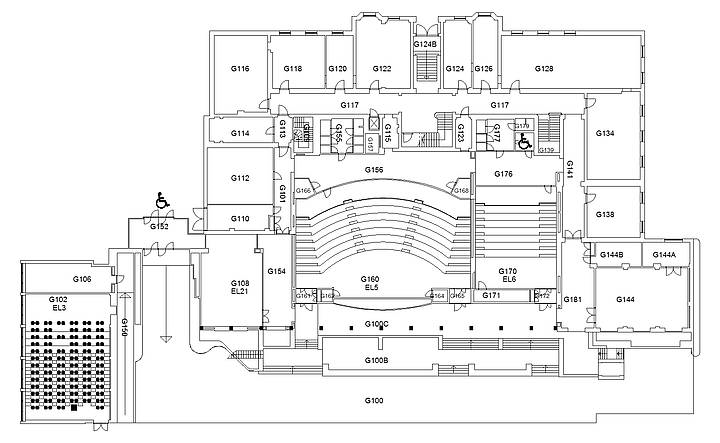
\includegraphics[width=\textwidth]{floorPlan}
		\caption{Floor plan of Gamle Elektro, first floor.}
		\label{fig:floorPlan}
	\end{subfigure}
	\caption{Comparison between mapped occupancy grid and floor plan.}\label{fig:comparison}
\end{figure}



\begin{figure}[h]
	\centering
	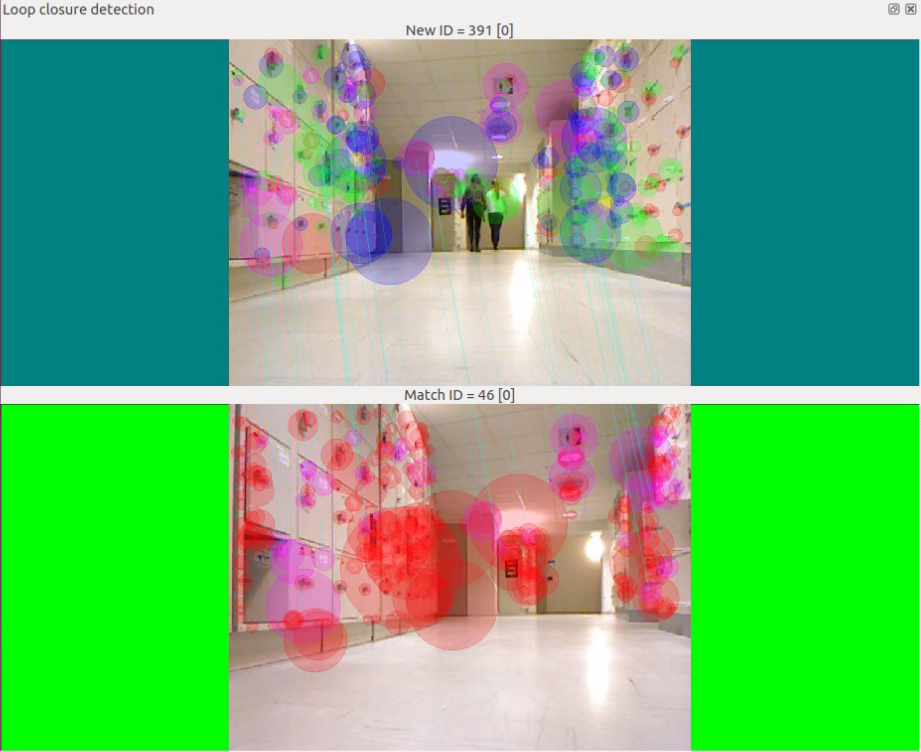
\includegraphics[width=1\textwidth]{lc_match_live}
	\caption{An example of an accepted loop closure hypothesis. This example is from the ''Asphalt'' world simulated in Gazebo.}
	\label{fig:lc_match_live}
\end{figure}

\begin{figure}[p]
	\centering
	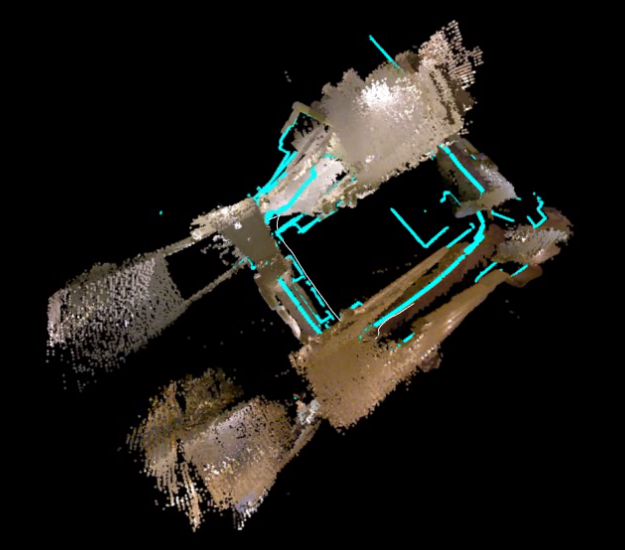
\includegraphics[width=1\textwidth]{lc_match_live_map}
	\caption{The resulting 3D map of the same area as in figure \ref{fig:mapping_gamle_elektro}.}
	\label{fig:lc_match_live_map}
\end{figure}

\subsubsection{Multi Session Mapping}

Multi session mapping was tested by performing an initial mapping run and then starting a second mapping session from an unknown location. All multi session mapping trials were successful. 

\subsubsection{Navigating Among Static Obstacles}

The first live navigation trials were performed by setting up a static obstacle course in a hallway. Only a few people were using this hallway, so multiple trials could be carried in under similar conditions. Most navigation trials were carried out in mapped areas. The robot performed well when navigating in known environments. In unknown environments, the robot will still plan a path. 



\subsubsection{Avoiding Moving Obstacles}

The navigation stack is configured to use a static global map for global planning and a local cost map that is linked with the mobile base and is based on real time sensor data. The local cost map will receive LIDAR laser scans, Kinect point clouds and point clouds representing detected obstacles detected by \texttt{rtabmap}. Being a real-time map, the local cost map should enable the local planner to avoid people and other non-static obstacles.

Moving obstacle avoidance testing was performed by having a person move into the planned path of the robot at different distances. Other avoidance situations would occur randomly as people were walking by the robot in the hallways. Tests showed that the robot is able to avoid non-static obstacles if the obstacle is observed at a distance larger than $0.5 - 0.8 m$. Figure \ref{fig:obstacle_avoidance} shows that the robot has successfully planned a new path around a person. If an obstacle appeared any closer than this, the new circumnavigating plan would either be too close to the original plan or not be planned at all. Detection and planning was not instantaneous. Some time would pass before the obstacle was detected and a new local plan was generated. This detection delay reduced the detectability of people walking by the robot. Figure \ref{fig:avoiding_moving_obstacles} shows an example of when the local cost map was lagging behind the actual moving obstacle.



\begin{figure}[p]
	\centering
	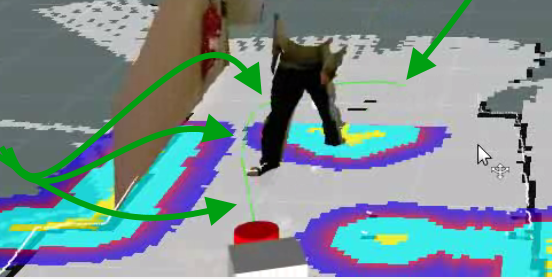
\includegraphics[width=1\textwidth]{avoiding_moving_obstacles_arrow}
	\caption{Avoiding moving obstacles with a new plan that circumnavigates the detected obstruction. In this situation, the obstacle was moving too fast for the local planner. The right leg is not yet registered as an obstacle.}
	\label{fig:avoiding_moving_obstacles}
\end{figure}

\begin{figure}
	\centering
	\begin{subfigure}[b]{0.46\textwidth}
		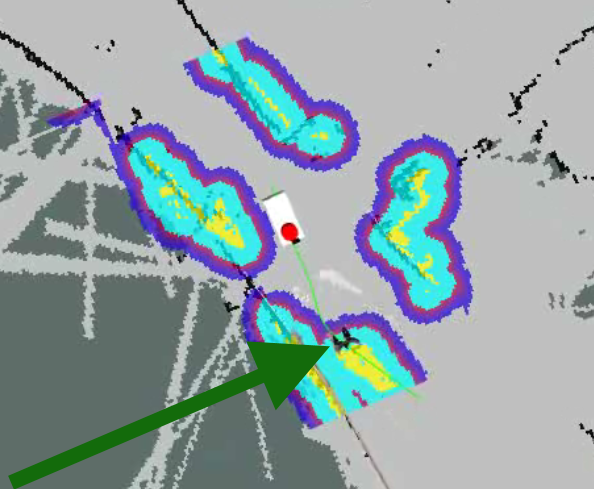
\includegraphics[width=\textwidth]{obstructed_plan_arrow}
		\caption{A person has moved into the path of the robot.}
		\label{fig:obstructed_plan}
	\end{subfigure}
	\begin{subfigure}[b]{0.472\textwidth}
		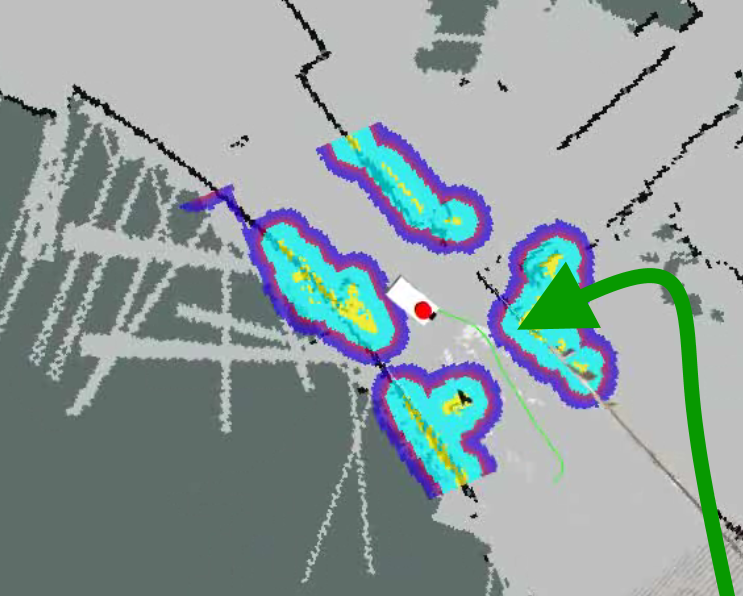
\includegraphics[width=\textwidth]{corrected_plan_arrow}
		\caption{A new path is planned, avoiding the new obstacle.}
		\label{fig:corrected_plan}
	\end{subfigure}
	\caption{Moving obstacle avoidance. The local cost map, shown as coloured spots on the occupancy grid, is based on real-time sensor data. }\label{fig:obstacle_avoidance}
\end{figure}




\section{Discussion}